\section{Introduction}

Deep networks can become highly over-parameterized, in the classical sense, and thus can approximate even randomly generated training data. Despite this capacity, they are typically arrive at solutions that generalise to unseen data in a way that cannot be accounted for by memorising the training. The development of complexity measures aims at investigating this phenomena in computationally tractable ways; with the intention on illuminating deep network training beyond loss curves, or providing tools the regularise the training process. In this chapter we explore how the tools of Part \ref{part:theoretical_foundations} can be utilised to construct complexity measures for deep networks.

\section{Local Complexity}\label{sec:local_complexity}

Let $V=\left(\mathbf{v}_1,\dots,\mathbf{v}_p\right)^\top$ be a matrix of vertices in a deep network's input space. Let $\mathcal{V}=\mathrm{conv}(V)$. Recall that the partition of the input space of layer $\ell$ can be expressed as the set of hyperplanes $$\partial\Omega=\bigcup_{i=1}^{d^{(\ell)}}\mathcal{H}^{(\ell)}_i,$$where $$\mathcal{H}^{(\ell)}_i=\left\{\mathbf{z}\in\mathbb{R}^{d^{(\ell-1)}}:\left\langle\left[W^{(\ell)}\right]_i,\mathbf{z}\right\rangle+\left[b^{(\ell)}\right]_i=0\right\}.$$One gauge the local complexity of $\mathcal{V}$ induced by layer $\ell$ by counting the number of regions in $$\mathcal{V}^{(\ell)}\cap\partial\Omega=\bigcup_{i=1}^{d^{(\ell)}}\mathcal{V}^{(\ell)}\cap\mathcal{H}^{(\ell)}_i,$$where $\mathcal{V}^{(\ell)}$ is the embedded representation of $\mathcal{V}$ after layer $\ell-1$ of the deep network. In particular, this will be on the order of $\mathcal{N}^{d^{(\ell-1)}}$, where $$\mathcal{N}=\left\vert\left\{i:i=1,\dots,d^{(\ell)}\text{ and }\mathcal{H}^{(\ell)}_i\cap\mathcal{V}^{(\ell)}\neq\emptyset\right\}\right\vert,$$which can thus be used as a proxy for the local complexity of $\mathcal{V}^{(\ell-1)}$. For practical tractability it is convenient to work with the convex hull of $V^{(\ell)}$\footnote{The matrix $\left(\mathbf{v}^{(1)},\dots,\mathbf{v}^{(p)}\right)^\top$, where $\mathbf{v}^{(\ell)}_i$ is the embedded representation of $\mathbf{v}_i$ after layer $\ell-1$ of the deep network.} which we will denote $\hat{\mathcal{V}}^{(\ell)}$.

\section{Absolute Deviation}\label{sec:absolute_deviation}

\subsection{Adaptive Linear Region Discovery}

For a hyperplane $\mathcal{H}^{(\ell)}_i\subseteq\mathbb{R}^{d^{(\ell-1)}}$, suppose that $\mathbf{z}^{(\ell-1)}(\mathbf{x})$ lies on its negative side.\footnote{If $\mathbf{z}^{(\ell-1)}(\mathbf{x})$ is on the positive side, flip the inequality and sign of $\lambda^{(\ell)}_j$ in \eqref{eq:adaptive_linear_region_min_problem}.}Then the smallest displacement $\lambda^{(\ell)}_j$ along a direction $\mathbf{d}\in\mathbb{R}^{d}$, that is non-zero and not lying in $\mathcal{H}^{(\ell)}_j$, required to cross $\mathcal{H}^{(\ell)}_j$ is
\begin{align}\label{eq:adaptive_linear_region_min_problem}
    \lambda^{(\ell)}_j&=\min_{\lambda\in\mathbb{R}}\left(\left[W^{(\ell)}\right]_{j,\cdot}^\top\left(\mathbf{z}^{(\ell-1)}+\lambda\mathbf{d}^{(\ell)}\right)+\left[b^{(\ell)}\right]_j>0\right)\nonumber\\&=\min_{\lambda\in\mathbb{R}}\left(\lambda>\frac{-\left[W^{(\ell)}\right]_{j,\cdot}^\top\mathbf{z}^{(\ell-1)}-\left[b^{(\ell)}\right]_j}{\left[W^{(\ell)}\right]_{j,\cdot}^\top\mathbf{d}^{(\ell)}}\right),
\end{align}
where $\mathbf{d}^{(\ell)}\in\mathbb{R}^{d^{(\ell-1)}}$ is the direction $\mathbf{d}$ in the input space of layer $\ell$, namely $\mathbf{d}^{(\ell)}=A_{\omega_{\mathbf{s}^{(1\leftarrow\ell)}\left(\mathbf{x}\right)}}^{(1\leftarrow\ell)}\mathbf{d}$.

In practice, the condition $\vert\lambda\vert>\tau$ for a sensitivity parameter $0<\tau\ll1$ is added to \eqref{eq:adaptive_linear_region_min_problem}, to ensure that a sufficient step is taken along $\mathbf{d}$ to traverse the boundary.

\begin{algorithm}
\caption{Minimum displacement finder.}\label{alg:min_displacement_finder}
\begin{algorithmic}
\Require $\mathbf{x}$, $\mathbf{d}$
\For{$\ell=1,\dots,L$}
\State $\lambda\leftarrow\infty$.
\State $\text{lambdas}\leftarrow\emptyset$.
\State $\text{lambdas}\leftarrow\frac{-b^{(\ell)}-W^{(\ell)}\mathbf{x}}{W^{(\ell)}\mathbf{d}}$. \Comment{Division is element-wise.}
\If{$\min(\text{lambdas})<\lambda$}
\State $\lambda\leftarrow\min(\text{lambdas})$.
\EndIf
\State $\mathbf{x}\leftarrow A^{(\ell)}_{\omega_{\mathbf{s}^{(\ell)}\left(\mathbf{x}\right)}}\mathbf{x}+b^{(\ell)}_{\omega_{\mathbf{s}^{(\ell)}\left(\mathbf{x}\right)}}$.
\State $\mathbf{d}\leftarrow A^{(\ell)}_{\omega_{\mathbf{s}^{(\ell)}\left(\mathbf{x}\right)}}\mathbf{d}$.
\EndFor
\State \Return $\text{lambdas}$.
\end{algorithmic}
\end{algorithm}

Given a $\mathbf{x}\in\mathbb{R}^d$ and a direction $\mathbf{d}$, the smallest displacement $\lambda$ in direction $\mathbf{d}$ to a region is given by iteratively solving \eqref{eq:adaptive_linear_region_min_problem} for each layer, namely $$\lambda=\min_{1\leq\ell\leq L,1\leq j\leq d^{(\ell-1)}}\lambda_j^{(\ell)},$$as summarised in Algorithm \ref{alg:min_displacement_finder}.

Iterating this procedure, it is possible to discover all regions along a path $\boldsymbol{\pi}:[0,1]\to\mathbb{R}^d$ given by $\boldsymbol{\pi}(t)=\mathbf{x}+t\mathbf{d}$. Since by the convexity of the regions, they induce a partition 
\begin{equation}\label{eq:path_region_partition}
    \mathcal{P}=\left\{t\in[0,1]:0=t_0<\dots<t_n=1\right\}.
\end{equation}
Letting $\mathcal{J}_i=\left[t_i,t_{i+1}\right]$, it follows that with $\tau<\min_{i=1,\dots,n}\left\vert\mathcal{J}_i\right\vert$ Algorithm \ref{alg:alrd_one_d} recovers all the regions, otherwise it recovers the regions with size larger than $\tau$.

\begin{algorithm}
\caption{Adaptive linear region discovery on compact one-dimensional domains.}\label{alg:alrd_one_d}
\begin{algorithmic}
\Require $\mathbf{x}_0$, $\mathbf{x}_1$, $\tau$
\State $\mathbf{c}\leftarrow\mathbf{s}\left(f\left(\mathbf{x}_0\right)\right)$.\Comment{Computed element-wise.}
\State $\mathbf{c}_1\leftarrow\mathbf{s}\left(f\left(\mathbf{x}_1\right)\right)$.
\State $\mathbf{d}\leftarrow\frac{\mathbf{x}_1-\mathbf{x}_0}{\left\Vert\mathbf{x}_1-\mathbf{x}_0\right\Vert_2}$.
\State $\mathcal{P}\leftarrow\emptyset$.
\While{$\mathbf{c}\neq\mathbf{c}_1$}
\State $\lambda\leftarrow$ Algorithm \ref{alg:min_displacement_finder}$(\mathbf{x},\mathbf{d})$.
\State $\mathcal{P}\leftarrow\mathcal{P}\cup\{\lambda\}$.
\If{$\lambda=\infty$}
\State \textbf{break}
\EndIf
\State $\mathbf{x}\leftarrow\mathbf{x}+\lambda\mathbf{d}$.
\If{$\left\Vert\mathbf{x}_0-\mathbf{x}_1\right\Vert_2<\left\Vert\mathbf{x}-\mathbf{x}_0\right\Vert_2$}
\State \textbf{break}
\EndIf
\State $\mathbf{c}\leftarrow\mathbf{s}(f(\mathbf{x}))$.
\EndWhile
\State \Return $\mathcal{P}$.
\end{algorithmic}
\end{algorithm}

\subsection{Quantifying Nonlinearity}

For distinct points $\mathbf{x}_0,\mathbf{x}_1\in\mathbb{R}^d$ let $g$ be an interpolation of $f_{\omega_{\mathbf{s}\left(\mathbf{x}_0\right)}}$ and $f_{\omega_{\mathbf{s}\left(\mathbf{x}_1\right)}}$ such that $$g\left(\mathbf{x}_0+t\left(\mathbf{x}_1-\mathbf{x}_0\right)\right)=f\left(\mathbf{x}_0\right)+t\left(f\left(\mathbf{x}_1\right)-f\left(\mathbf{x}_0\right)\right).$$

\begin{definition}
    The absolute deviation between distinct points $\mathbf{x}_0,\mathbf{x}_1\in\mathbb{R}^d$ is $$\mathbf{a}\left(\mathbf{x}_0,\mathbf{x}_1\right)=\int_{\pi}\left\vert f(\mathbf{x})-g(\mathbf{x})\right\vert\,\mathrm{d}\mathbf{x},$$where $\boldsymbol{\pi}:[0,1]\to\mathbb{R}^d$ is given by $\boldsymbol{\pi}(t)=\mathbf{x}_0+t\left(\mathbf{x}_1-\mathbf{x}_0\right)$.\footnote{In practice, often the $\ell_2$ norm of $\mathbf{a}\left(\mathbf{x}_0,\mathbf{x}_1\right)$ is considered instead as a scalar score.} 
\end{definition}

\begin{figure}
    \centering
    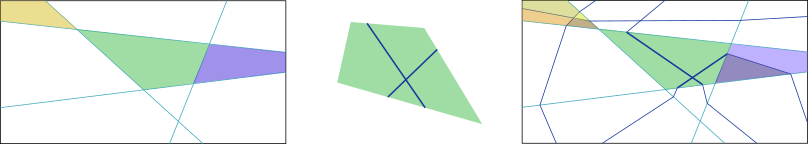
\includegraphics[width=0.75\linewidth]{drawings/iterative_partitioning_procedure.png}
    \caption{An illustration of what our notation for absolute deviation means in the context deep networks with a one-dimensional input domain. The region shaded in green represents the absolute deviation.}
    \label{fig:absolute_deviation}
\end{figure}

\begin{proposition}
    Recall that a deep network's regions induces a partition on $[0,1]$ \eqref{eq:path_region_partition}. For $j=1,\dots,d^{(L)}$ we have
    \begin{align*}
        \int_{\boldsymbol{\pi}}\left\vert\left[f(\mathbf{x})\right]_j-\left[\mathbf{a}(\mathbf{x})\right]_j\right\vert\,\mathrm{d}\mathbf{x}=\Vert\mathbf{d}\Vert\Bigg(\sum_{i=0}^{n-1}&\left(t_{\star}-t_i\right)\left\vert\left[f_{\omega_i}\left(\mathbf{x}_0\right)\right]_j-\left[f_{\omega_0}\left(\mathbf{x}_0\right)\right]_j\right\vert\\+&\left(t_{i+1}-t_{\star}\right)\left\vert\left[f_{\omega_i}\left(\mathbf{x}_0\right)\right]_j-\left[f_{\omega_0}\left(\mathbf{x}_0\right)\right]_j\right\vert\\+&\frac{t_{\star}^2-t_i^2}{2}\left\vert\left[f_{\omega_i}\left(\mathbf{x}_1\right)\right]_j-\left[f_{\omega_i}\left(\mathbf{x}_0\right)\right]_j-\left[f_{\omega_1}\left(\mathbf{x}_1\right)\right]_j+\left[f_{\omega_0}\left(\mathbf{x}_0\right)\right]_j\right\vert\\+&\frac{t_{i+1}^2-t_{\star}^2}{2}\left\vert\left[f_{\omega_i}\left(\mathbf{x}_1\right)\right]_j-\left[f_{\omega_i}\left(\mathbf{x}_0\right)\right]_j-\left[f_{\omega_1}\left(\mathbf{x}_1\right)\right]_j+\left[f_{\omega_0}\left(\mathbf{x}_0\right)\right]_j\right\vert\Bigg),
    \end{align*}
    where $t_{\star}=\max\left(t_i,\min\left(z_i,t_{i+1}\right)\right)$ for $$z_i=\frac{\left[f_{\omega_0}\left(\mathbf{x}_0\right)\right]_j-\left[f_{\omega_i}\left(\mathbf{x}_0\right)\right]_j}{\left[f_{\omega_i}\left(\mathbf{x}_1\right)\right]_j-\left[f_{\omega_i}\left(\mathbf{x}_0\right)\right]_j-\left[f_{\omega_1}\left(\mathbf{x}_1\right)\right]_j-\left[f_{\omega_0}\left(\mathbf{x}_0\right)\right]_j},$$and where $f_{\omega_i}$ denotes the affine function of the deep network operating on the region corresponding to $t_i$ in $\mathcal{P}$.
\end{proposition}

\begin{tproof}
    Initially, we obtain that
    \begin{align*}
        \int_{\boldsymbol{\pi}}&\left\vert\left[f(\mathbf{x})\right]_j-\left[\mathbf{a}(\mathbf{x})\right]_j\right\vert\,\mathrm{d}\mathbf{x}\\&=\sum_{i=0}^{n-1}\int_{t_i}^{t_{i+1}}\left\vert\left[f(\boldsymbol{\pi}(t))\right]_j-\left[\mathbf{a}(\boldsymbol{\pi}(t))\right]_j\right\vert\left\Vert\dot{\boldsymbol{\pi}}(t)\right\Vert\,\mathrm{d}t\\&=\sum_{i=0}^{n-1}\int_{t_i}^{t_{i+1}}\left\vert\left[f\left(\mathbf{x}_0+t\mathbf{d}\right)\right]_j-\left[\mathbf{a}\left(\mathbf{x}_0+t\mathbf{d}\right)\right]_j\right\vert\Vert\mathbf{d}\Vert\,\mathrm{d}t\\&=\Vert\mathbf{d}\Vert\sum_{i=0}^{n-1}\int_{t_i}^{t_{i+1}}\left\vert\left[f_{\omega_i}\left(\mathbf{x}_0\right)\right]_j-\left[f_{\omega_0}\left(\mathbf{x}_0\right)\right]_j+t\left(\left[f_{\omega_i}\left(\mathbf{x}_1\right)\right]_j-\left[f_{\omega_i}\left(\mathbf{x}_0\right)\right]_j-\left[f_{\omega_1}\left(\mathbf{x}_1\right)\right]_j+\left[f_{\omega_0}\left(\mathbf{x}_0\right)\right]_j\right)\right\vert\,\mathrm{d}t.
    \end{align*}
    Now the integrand is not necessarily monotonic, in particular, on $\omega_i$ the functions $\left[f\right]_j$ and $\left[\mathbf{a}\right]$ may intersect at $$z_i=\frac{\left[f_{\omega_0}\left(\mathbf{x}_0\right)\right]_j-\left[f_{\omega_i}\left(\mathbf{x}_0\right)\right]_j}{\left[f_{\omega_i}\left(\mathbf{x}_1\right)\right]_j-\left[f_{\omega_i}\left(\mathbf{x}_0\right)\right]_j-\left[f_{\omega_1}\left(\mathbf{x}_1\right)\right]_j-\left[f_{\omega_0}\left(\mathbf{x}_0\right)\right]_j}.$$If $z_i\not\in\left(t_i,t_{i+1}\right)$, then we need not worry about this intersection for the computation of the integral, otherwise we can separate the integral across the domains $\left[t_i,z_i\right]$ and $\left[z_i,t_{i+1}\right]$. In any case, we can take $t_{\star}=\max\left(t_i,\min\left(z_i,t_{i+1}\right)\right)$ and consider the integral over the domains $\left[t_i,t_{\star}\right]$ and $\left[t_{\star},t_{i+1}\right]$ on which our integrand will be affine. Therefore,
    \begin{align*}
        \int_{\boldsymbol{\pi}}&\left\vert\left[f(\mathbf{x})\right]_j-\left[\mathbf{a}(\mathbf{x})\right]_j\right\vert\,\mathrm{d}\mathbf{x}\\&=\Vert\mathbf{d}\Vert\sum_{i=0}^{n-1}\int_{t_i}^{t_{\star}}\left\vert\left[f_{\omega_i}\left(\mathbf{x}_0\right)\right]_j-\left[f_{\omega_0}\left(\mathbf{x}_0\right)\right]_j+t\left(\left[f_{\omega_i}\left(\mathbf{x}_1\right)\right]_j-\left[f_{\omega_i}\left(\mathbf{x}_0\right)\right]_j-\left[f_{\omega_1}\left(\mathbf{x}_1\right)\right]_j+\left[f_{\omega_0}\left(\mathbf{x}_0\right)\right]_j\right)\right\vert\,\mathrm{d}t\\&+\Vert\mathbf{d}\Vert\sum_{i=0}^{n-1}\int_{t_{\star}}^{t_{i+1}}\left\vert\left[f_{\omega_i}\left(\mathbf{x}_0\right)\right]_j-\left[f_{\omega_0}\left(\mathbf{x}_0\right)\right]_j+t\left(\left[f_{\omega_i}\left(\mathbf{x}_1\right)\right]_j-\left[f_{\omega_i}\left(\mathbf{x}_0\right)\right]_j-\left[f_{\omega_1}\left(\mathbf{x}_1\right)\right]_j+\left[f_{\omega_0}\left(\mathbf{x}_0\right)\right]_j\right)\right\vert\,\mathrm{d}t,
    \end{align*}
    which simplifies to the desired expression.
\end{tproof}

\section{Hessian Based Rugosity Measure}\label{sec:hessian_rugosity}

Throughout this section we'll be consider a deep network $f:\mathbb{R}^d\to\mathbb{R}$ and a set of training data $\left\{\left(\mathbf{x}_i,y_i\right)\right\}_{i=1}^n$ where $\mathbf{x}_i\in\mathbb{R}^d$ and $y_i\in\mathbb{R}$ for $i=1,\dots,n$. In particular, we assume that the points $\left\{\mathbf{x}_i\right\}_{i=1}^n$ lie close to an $m$-dimensional manifold $\mathcal{M}\subseteq\mathbb{R}^d$.

\subsection{Smooth Activation Deep Networks}

Suppose that $f$ employs smooth activation operators. For $p\geq1$ let $$C_p(f):=\left(\int_{\mathcal{M}}\left\Vert\nabla^2_{\text{tan}}f(\mathbf{x})\right\Vert^p_F\,\mathrm{d}\mathbf{x}\right)^{\frac{1}{p}},$$where $\nabla^2_{\text{tan}}f(\mathbf{x})$ is the Hessian of $f$ at $\mathbf{x}$ in the coordinates of the $m$-dimensional affine space tangent to the manifold at $\mathbf{x}\in\mathcal{M}$.

The quantity $C_p(f)$ measure the average \emph{curviness} of $f$ over $\mathcal{M}$. More specifically, it is zero if and only if $f$ is an affine function on $\mathcal{M}$.

As $f$ is smooth, we have $$\nabla^2f(\mathbf{x})\mathbf{u}=\lim_{\epsilon\to0}\left(\frac{\nabla f(\mathbf{x}+\epsilon\mathbf{u})-\nabla f(\mathbf{x})}{\epsilon}\right).$$Moreover, for $\mathbf{u}\in\mathbb{R}^d$ chosen uniformly at random on the unit sphere, we have $$\mathbb{E}\left(\left\Vert A\mathbf{u}\right\Vert_2^2\right)=\mathbb{E}\left(\sum_{i,j=1,\dots,d}[\mathbf{u}]_i[\mathbf{u}]_j\left[A^\top A\right]_{ij}\right)=\frac{\Vert A\Vert_F^2}{d},$$for any $A\in\mathbb{R}^{d\times d}$. Therefore, we can obtain a Monte Carlo approximation for $C_p(f)$ on the training data as $$\tilde{C}_{p,\epsilon}(f)=\left(\frac{d^{\frac{p}{2}}}{n\epsilon^p\hat{n}^{\frac{p}{2}}}\sum_{i=1}^n\left(\sum_{j=1}^{\hat{n}}\left\Vert\nabla f\left(\mathbf{x}_i+\epsilon\mathbf{u}_j\right)-\nabla f\left(\mathbf{x}_i\right)\right\Vert_2^2\right)\right)^{\frac{1}{p}},$$where $\epsilon>0$ is small and the $\mathbf{u}_j$ are uniform samples of unit vectors on the $m$-dimensional subspace tangent to $\mathcal{M}$ at $\mathbf{x}$. This just follows from the observation that $$$$

\subsection{Continuous Piecewise Affine Deep Networks}

For $f$ employing piecewise affine activation operators, it can be characterised as a continuous piecewise affine operator. In particular, recall the notation convention from statement 2 of Remark \ref{rem:affine_spline}, we have that $f(\mathbf{x})=A[\mathbf{x}]\mathbf{x}+b[\mathbf{x}]$, where $A[\mathbf{x}]$ and $b[\mathbf{x}]$ are the parameters for the affine function on the region encompassing $\mathbf{x}$.

The Hessian for $f$ is not well-defined, however, we can extend a definition of the Hessian to encompass this case. Let $\epsilon>0$. Then for $\mathbf{x}\in\mathbb{R}^d$ not on the boundary of a partition and a unit vector $\mathbf{u}$, let $$H^{\epsilon}_{\mathbf{u}}(\mathbf{x})=\begin{cases}\frac{A\left[\mathbf{x}+\epsilon\mathbf{u}\right]-A[\mathbf{x}]}{\epsilon}&\mathbf{u}\text{ in tangent manifold of }\mathcal{M}\text{ at }\mathbf{x}\\\mathbf{0}&\text{otherwise}.\end{cases}$$With this, for $p\geq1$, let $$C_{p,\epsilon}:=\sqrt{d}\left(\int_{\mathcal{M}}\left(\mathbb{E}_{\mathbf{u}}\left(\left\Vert H_{\mathbf{u}}^{\epsilon}(\mathbf{x})\right\Vert_2^2\right)\right)^{\frac{p}{2}}\right)^{\frac{1}{p}},$$where $\mathbf{u}$ is uniform over the unit sphere.

A Monte Carlo approximation for $C_{p,\epsilon}(f)$ on the training data can be obtained as 
\begin{equation}\label{eq:monte_carlo_rugosity_cpa}
    \tilde{C}_{p,\epsilon}(f)=\left(\frac{d^{\frac{p}{2}}}{n\epsilon^p\hat{n}^{\frac{p}{2}}}\sum_{i=1}^n\left(\sum_{j=1}^{\hat{n}}\left\Vert A\left[\mathbf{x}_i+\epsilon\mathbf{u}_j\right]-A\left[\mathbf{x}_i\right]\right\Vert_2^2\right)\right)^{\frac{1}{p}},
\end{equation}
where the $\mathbf{u}_j$ are uniform samples of unit vectors on the $m$-dimensional subspace tangent to $\mathcal{M}$ at $\mathbf{x}$.

\subsection{Connection to Data Augmentation}

The process of data augmentation takes the original dataset $\left\{\left(\mathbf{x}_i,y_i\right)\right\}_{i=1}^n$ and generates the augmented dataset $\left\{\left\{\left(\mathbf{x}_i+\mathbf{u}_{ij},y_i\right)\right\}_{j=0}^{\hat{n}}\right\}_{i=1}^n$ by applying transformations to the points $\mathbf{x}_i$ such that they continue to lie on $\mathcal{M}$. In this case, we are using $\mathbf{u}_{i0}$ to represent the identity transformation on $\mathbf{x}_i$. Training $f$ on the original dataset involves minimizing a loss $$\mathcal{L}:=\sum_{i=1}^\ell\left(f\left(\mathbf{x}_i\right),y_i\right),$$where we are assuming $\ell$ is convex. On the augmented dataset the corresponding loss is $$\mathcal{L}_{\text{aug}}:=\frac{1}{\hat{n}+1}\sum_{i=1}^n\left(\ell\left(f\left(\mathbf{x}_i\right),y_i\right)+\sum_{j=1}^{\hat{n}}\ell\left(f\left(\mathbf{x}_i+\mathbf{u}_{ij}\right),y_i\right)\right).$$

\begin{theorem}
    Let $f$ be a deep network that is a continuous piecewise affine operator. Assume that $\left\Vert\mathbf{x}_i\right\Vert_2\leq R$, that $f$ has Lipschitz constant $K_1$, and that $\ell$ has Lipschitz constant $K_2$. Then for $\left\Vert\mathbf{u}_{ij}\right\Vert_2\leq\epsilon$ we have 
    \begin{align}
        \mathcal{L}_{\text{aug}}\leq\mathcal{L}&+\frac{RK_2}{\hat{n}+1}\underbrace{\sum_{i=1}^n\sum_{j=1}^{\hat{n}}\left\Vert A\left[\mathbf{x}_i+u_{ij}\right]-A\left[\mathbf{x}_i\right]\right\Vert_2}_{\hat{C}(f)}\nonumber\\&+\frac{K_2}{\hat{n}+1}\sum_{i=1}^n\sum_{j=1}^{\hat{n}}\left\vert b\left[\mathbf{x}_i+\mathbf{u}_{ij}\right]-b\left[\mathbf{x}_i\right]\right\vert\nonumber\\&+\frac{K_1K_2\hat{n}n\epsilon}{\hat{n}+1}+o(\epsilon).
    \end{align}
\end{theorem}

\begin{tproof}
    Observe that
    \begin{align*}
        \ell\left(f\left(\mathbf{x}_i+\mathbf{u}_{ij}\right),y_i\right)&=\ell\left(A\left[\mathbf{x}_i+\mathbf{u}_{ij}\right]\left(\mathbf{x}_i+\mathbf{u}_{ij}\right)+b\left[\mathbf{x}_i+\mathbf{u}_{ij}\right],y_i\right)\\&=\ell\big(A\left[\mathbf{x}_i\right]\mathbf{x}_i+b\left[\mathbf{x}_i\right]+\left(A\left[\mathbf{x}_i+\mathbf{u}_{ij}\right]-A\left[\mathbf{x}_i\right]\right)\mathbf{x}_i\\&\qquad+\left(b\left[\mathbf{x}_i+\mathbf{u}_{ij}\right]-b\left[\mathbf{x}_i\right]\right)+A\left[\mathbf{x}_i+\mathbf{u}_{ij}\right]\mathbf{u}_{ij},y_i\big).
    \end{align*}
    Therefore, the first-order approximation of $\ell\left(f\left(\mathbf{x}_i+\mathbf{u}_{ij}\right),y_i\right)$ around $\ell\left(f\left(\mathbf{x}_ir\right),y_i\right)$ is 
    \begin{align*}
        \tilde{\ell}\left(f\left(\mathbf{x}_i+\mathbf{u}_{ij}\right),y_i\right)=&\ell\left(f\left(\mathbf{x}_ir\right),y_i\right)\\&+\big(\left(A\left[\mathbf{x}_i+\mathbf{u}_{ij}\right]-A\left[\mathbf{x}_i\right]\right)\mathbf{x}_i\\&\qquad+\left(b\left[\mathbf{x}_i+\mathbf{u}_{ij}\right]-b\left[\mathbf{x}_i\right]\right)+A\left[\mathbf{x}_i+\mathbf{u}_{ij}\right]\mathbf{u}_{ij}\big)^\top\nabla_{f\left(\mathbf{x}_i\right)}\ell\left(f\left(\mathbf{x}_i\right),y_i\right).
    \end{align*}
    Hence, 
    \begin{align*}
        \tilde{\ell}\left(f\left(\mathbf{x}_i+\mathbf{u}_{ij}\right),y_i\right)\leq&\ell\left(f\left(\mathbf{x}_ir\right),y_i\right)+RK_2\left\Vert A\left[\mathbf{x}_i+\mathbf{u}_{ij}\right]-A\left[\mathbf{x}_i\right]\right\Vert_2\\&+K_2\left\vert b\left[\mathbf{x}_i+\mathbf{u}_{ij}\right]-b\left[\mathbf{x}_i\right]\right\vert+\epsilon K_1K_2.
    \end{align*}
    Therefore, 
    \begin{align*}
        \tilde{\mathcal{L}}_{\text{aug}}&=\frac{1}{\hat{n}+1}\sum_{i=1}^n\left(\ell\left(f\left(\mathbf{x}_ir\right),y_i\right)+\sum_{j=1}^{\hat{n}}\tilde{\ell}\left(f\left(\mathbf{x}_i+\mathbf{u}_{ij}\right),y_i\right)\right)\\&\leq\mathcal{L}+\frac{RK_2}{\hat{n}+1}\sum_{i=1}^n\sum_{j=1}^{\hat{n}}\left\Vert A\left[\mathbf{x}_i+\mathbf{u}_{ij}\right]-A\left[\mathbf{x}_i\right]\right\Vert_2\\&\quad+\frac{K_2}{\hat{n}+1}\sum_{i=1}^n\sum_{j=1}^{\hat{n}}\left\vert b\left[\mathbf{x}_i+\mathbf{u}_{ij}\right]-b\left[\mathbf{x}_i\right]\right\vert+\frac{K_1K_2n\hat{n}\epsilon}{\hat{n}+1},
    \end{align*}
    completing the proof.
\end{tproof}

\begin{remark}
    Note how for $p=1$, \eqref{eq:monte_carlo_rugosity_cpa} is very similar to $\hat{C}(f)$, up to a normalisation constant. Moreover, the data augmentations methods are such that $\mathbf{x}_i+\mathbf{u}_{ij}\in\mathcal{M}$. Thus, a sufficiently rich set of small augmentations will have similar distribution and support to the uniform distribution over unit vectors on the subspace tangent to the manifold, as is the case in \eqref{eq:monte_carlo_rugosity_cpa}. Therefore, the Hessian-based rugosity measure \eqref{eq:monte_carlo_rugosity_cpa} could act as an explicit regularisation term in training that yields similar benefits as data augmentation, namely minimising $\mathcal{L}_{\text{aug}}$.
\end{remark}

\section{References}

Section \ref{sec:local_complexity} from \citet{humayunDeepNetworksAlways2024}. Section \ref{sec:absolute_deviation} from \citet{gambaAreAllLinear2022}. Section \ref{sec:hessian_rugosity} from \citet{lejeuneImplicitRugosityRegularization2019}.